\documentclass[spanish]{textolivre}

% metadata
\journalname{Texto Livre}
\thevolume{17}
%\thenumber{1} % old template
\theyear{2024}
\receiveddate{\DTMdisplaydate{2024}{2}{11}{-1}}
\accepteddate{\DTMdisplaydate{2024}{5}{20}{-1}}
\publisheddate{\DTMdisplaydate{2024}{5}{31}{-1}}
\corrauthor{Karla Karina Ruiz Mendoza}
\articledoi{10.1590/1983-3652.2024.51222}
%\articleid{NNNN} % if the article ID is not the last 5 numbers of its DOI, provide it using \articleid{} commmand 
% list of available sesscions in the journal: articles, dossier, reports, essays, reviews, interviews, editorial
\articlesessionname{articles}
\runningauthor{Ruiz Mendoza et al.}
%\editorname{Leonardo Araújo} % old template
\sectioneditorname{Hugo Heredia Ponce}
\layouteditorname{João Mesquita}

\title{Creación y jueceo de ítems: ChatGPT como diseñador y juez}
\othertitle{Criação e julgamento de itens: ChatGPT como designer e juiz}
\othertitle{Item creation and judging: ChatGPT as designer and judge}

\author[1]{Karla Karina Ruiz Mendoza~\orcid{0000-0001-8978-8364}\thanks{Email: \href{mailto:ruiz.karla32@uabc.edu.mx}{ruiz.karla32@uabc.edu.mx}}}
\author[1]{Luis Horacio Pedroza Zúñiga~\orcid{0000-0002-5256-2967}\thanks{Email: \href{mailto:horacio.pedroza@uabc.edu.mx}{horacio.pedroza@uabc.edu.mx}}}
\author[2]{Alma Yadhira López García~\orcid{0000-0002-7474-5799}\thanks{Email: \href{mailto:alma.l@thelearningbar.com}{alma.l@thelearningbar.com}}}
\affil[1]{Universidad Autónoma de Baja, California, IIDE, Ensenada, Baja California, México.}
\affil[2]{TheLearning Bar, Canadá.}

\addbibresource{article.bib}
\usepackage{array,longtable,multirow}
\usepackage{enumitem}


\begin{document}
\maketitle
\begin{polyabstract}
\begin{abstract}
El fin de este estudio fue evaluar la efectividad de la inteligencia
artificial (IA), representada por ChatGPT 4.0, comparada con diseñadores
humanos en la creación de ítems para un examen para el ingreso a la
educación superior en el área de Lengua Escrita. Se utilizó un enfoque
mixto, combinando metodologías clásicas y contemporáneas en evaluación
educativa, incluyendo el juicio de expertos. ChatGPT y cuatro
diseñadores humanos desarrollaron 84 ítems, siguiendo la Taxonomía de
Anderson y Krathwohl para establecer el nivel de demanda cognitiva. Los
ítems fueron evaluados por dos jueces humanos y ChatGPT, utilizando una
rúbrica detallada que incluye claridad, neutralidad, formato, alineación
curricular y redacción. Los resultados mostraron una alta tasa de
aceptación sin cambios tanto para ítems de ChatGPT como para los
humanos, indicando una buena alineación con los estándares de
evaluación. Sin embargo, se observaron diferencias en la necesidad de
cambios menores y mayores propuestos por la rúbrica. El estudio concluye
que tanto la IA como los diseñadores humanos son capaces de generar
ítems de alta calidad, resaltando el potencial de la IA en el diseño de
ítems educativos.

\keywords{Inteligencia Artificial \sep Evaluación educativa \sep
	ChatGPT \sep Diseño de ítems \sep Jueceo}
\end{abstract}

\begin{portuguese}
\begin{abstract}
O objetivo deste estudo foi avaliar a eficácia da inteligência
artificial (IA), representada pelo ChatGPT 4.0, em comparação com
designers humanos na criação de itens para um exame de ingresso ao
ensino superior na área de Língua Escrita. Utilizou-se uma abordagem
mista, combinando metodologias clássicas e contemporâneas em avaliação
educacional, incluindo o julgamento de especialistas. O ChatGPT e quatro
designers humanos desenvolveram 84 itens, seguindo a Taxonomia de
Anderson e Krathwohl para estabelecer o nível de demanda cognitiva. Os
itens foram avaliados por dois juízes humanos e pelo ChatGPT, utilizando
uma rubrica detalhada que inclui clareza, neutralidade, formato,
alinhamento curricular e redação. Os resultados mostraram uma alta taxa
de aceitação sem mudanças tanto para itens do ChatGPT quanto para os
humanos, indicando um bom alinhamento com os padrões de avaliação. No
entanto, foram observadas diferenças na necessidade de mudanças menores
e maiores propostas pela rubrica. Conclui-se que tanto a IA quanto os
designers humanos são capazes de gerar itens de alta qualidade,
destacando o potencial da IA no design de itens educacionais.


\keywords{Inteligência Artificial \sep Avaliação educacional \sep ChatGPT \sep Design de itens \sep Julgamento}
\end{abstract}
\end{portuguese}

\begin{english}
\begin{abstract}
The purpose of this study was to evaluate the effectiveness of
artificial intelligence (AI), represented by ChatGPT 4.0, compared to
human designers in creating items for an exam for entry into higher
education in the area of Written Language. A mixed approach was
utilized, combining classic and contemporary methodologies in
educational evaluation including expert judgment. ChatGPT and four human
designers developed 84 items, following Anderson and
Krathwohl\textquotesingle s Taxonomy to establish the level of cognitive
demand. The items were evaluated by two human judges and ChatGPT, using
a detailed rubric that includes clarity, neutrality, format, curricular
alignment, and writing. The results showed a high rate of acceptance
without changes for both ChatGPT and human items, indicating good
alignment with the evaluation standards. However, differences were
observed in the need for minor and major changes proposed by the rubric.
The study concludes that both AI and human designers are capable of
generating high-quality items, highlighting the potential of AI in the
design of educational items.

\keywords{Artificial Intelligence \sep Educational assessment \sep
	ChatGPT \sep Item design \sep Judging Process}
\end{abstract}
\end{english}

\end{polyabstract}

\section{Introducción}\label{sec-introducción}

Desde la antigüedad, la narración de historias ha servido a los seres
humanos para transmitir información, jugando un papel fundamental en el
desarrollo de las sociedades y en la conservación del patrimonio
inmaterial y cultural de las mismas. Hoy en día, con el paso de los
siglos, los modelos clásicos de construcción de historias siguen estando
vigentes en diversos ámbitos como el cinematográfico, el televisivo o la
creación de videojuegos. La publicidad o la comunicación política
también recurren a las técnicas del \emph{Storytelling.}

En el ámbito de la educación, la narración tiene una gran presencia como
estrategia didáctica \cite{vergara_ramirez_narrar_2018}. La aplicación de técnicas de
\emph{Storytelling} mediadas por tecnología educativa son muy utilizadas
en el aula, dando lugar a métodos didácticos específicos como el
Aprendizaje Basado en Historias \cite{sanchez_rivas_experiencia_2023}.

El Aprendizaje Basado en Historias es un método activo que promueve la
investigación a partir de una historia (cuento, novela o película),
utilizando para el proceso diferentes recursos tecnológicos, como
\emph{Google Workspace} o \emph{Genially}. La secuencia didáctica parte
de la generación de un vínculo emocional hacia la historia y culmina con
un producto de aplicación del aprendizaje a partir de la creación de
historias propias \cite{sanchez-rivas_narrative-based_2022}.

En el plano didáctico, las estrategias metodológicas basadas en la
narración de historias y mediadas por tecnología presentan importantes
beneficios para el proceso de enseñanza y aprendizaje. Entre ellos, se
encuentran los siguientes:

\begin{itemize}
	\item
	Favorece la comprensión, ya que las historias pueden ser utilizadas
	para acercarnos a conceptos y temas complejos de una forma más fácil
	de entender mediante el empleo de metáforas, ejemplos y analogías
	\cite{isbell_effects_2004,lenhart_more_2020}.
	\item
	Fomenta la empatía, permitiendo a los receptores identificarse con las
	situaciones que se describen y poniéndose en el lugar de sus
	personajes \cite{bratitsis_digital_2016,skaraas_playing_2018,vaughan-lee_power_2019}.
	\item
	Estimula el análisis, la reflexión y el pensamiento crítico, a través
	de las diferentes perspectivas desde las que se plantean las
	situaciones narradas \cite{larry_crumbley_using_2000,young_introducing_1996}.
	\item
	Impulsa la creatividad, fomentando el uso de la imaginación, la
	recreación de espacios, argumentos y soluciones alternativas \cite{celume_fostering_2019,tabieh_effect_2021}.
\end{itemize}

En el contexto educativo actual, marcado por las tecnologías digitales,
los discursos narrativos en al aula se han ido redefiniendo hacia los
llamados \enquote{transmedia}. \textcite{dudacek_transmedia_2015} describe el transmedia como un proceso en el que elementos integrales de una ficción se comunican a través de diferentes canales de distribución para estructurar y contar una historia. A esto hay que sumarle el cambio metodológico que implican los métodos activos, como el Aprendizaje Basado en Proyectos, el
Aprendizaje Basado en Resolución de Problemas o el Aprendizaje
Cooperativo.

De esta nueva configuración de los escenarios didácticos basados en la
narración y la tecnología, se deriva la necesidad de generar una base de
conocimiento científico a partir de la cual fundamentar intervenciones
docentes que combinen el aprendizaje basado en historias y la
tecnología, y ampliar el conocimiento generado en torno a estos tópicos.

El objetivo de este artículo consiste en identificar y analizar
publicaciones científicas que aborden investigaciones y experiencias
didácticas basadas en la aplicación de una enseñanza a partir de
historias y mediada por recursos tecnológicos, de manera que las
conclusiones extraídas puedan servir de base a futuros estudios e
investigadores que pretendan aportar conocimiento a una línea de
investigación tan sustancial como la descrita, y que contribuyan a
mejorar las experiencias educativas.

Existe una amplia producción bibliográfica sobre el \emph{Storytelling}
y tecnología, aplicada principalmente a los campos de los individuos y
sociedades, y a la creación, teoría y crítica literaria. En lo que se
refiere a su vertiente educativa, dicha producción se centra en aspectos
como su utilidad para enseñar y asimilar conceptos \cite{alismail2015integrate,sadik2008digital}, fomentar la comprensión lectora \cite{al-shaye2021digital,bakar2019digital} y modelar y analizar estudios de casos reales, especialmente en
los ámbitos científicos y de la salud \cite{moreau_digital_2018,open2022digital,thompson_communicating_2018}.

Aunque la narración de historias siempre ha estado vinculada a la
pedagogía, la evolución de la tecnología y la aparición de nuevas
metodologías activas han influido en la redefinición y adaptación de las
técnicas de narración en los procesos de enseñanza y aprendizaje. Desde
principios del siglo XXI se ha observado un gran interés por la
mediación tecnológica en la narración de historias en el ámbito
educativo, especialmente por la mayor capacidad de las técnicas visuales
y auditivas para captar la atención de los estudiantes frente a la
comunicación escrita \cite{suwardy2013using}. Entre sus principales
beneficios, numerosos estudios han destacado la flexibilidad de la
narración digital para integrar mensajes instructivos, crear entornos de
aprendizaje más atractivos, fomentar la reflexión, el trabajo en equipo
y el debate \cite{beck2021digital,smeda2014effectiveness,tiba2015digital}. Fruto de estos hallazgos han surgido diversas iniciativas
académicas como la creación del \enquote{Centro de Narrativa Digital} por
parte de la Universidad de Berkeley, California (Estados Unidos), que
establece claves y elementos de éxito para construir narrativas
digitales eficaces \cite{robin2008effective}, o la plataforma creada por la Facultad
de Educación de la Universidad de Houston, Texas (Estados Unidos)
destinada a recopilar y ofrecer recursos a educadores interesados en
integrar las narrativas digitales en sus actividades educativas
\cite{rudnicki2006buzz}.

Aprovechar la producción científica resulta esencial para identificar
problemas y establecer posibles soluciones que nos permitan mejorar y
abordar nuevos retos en el futuro. Por ello, se considera pertinente
ofrecer a la comunidad científica este trabajo de revisión, un análisis
que recoge las principales ideas que han aportado otros científicos e
investigadores.

En la actualidad, la comunidad científica dispone de numerosas bases de
datos que permiten revisar, analizar y contrastar la producción y el
trabajo realizado en diferentes campos de investigación. Sin embargo, la
gran cantidad de archivos bibliográficos disponibles sobre cualquier
objeto de estudio requiere un cuidadoso filtrado, dirigido a optimizar
el provecho de la investigación en curso. Esta necesidad ya ha sido
señalada por diversos autores \cite{baas_scopus_2020,schotten_brief_2017,vila_gamificacion_2019} que también destacan las ventajas de SCOPUS frente a
otras bases de datos. Entre ellas, debemos señalar la mayor cobertura
global en investigación, la relevancia e impacto de las publicaciones,
así como herramientas que facilitan el seguimiento, el análisis y la
visualización de las investigaciones, como factores clave para la
utilización de SCOPUS en este trabajo \cite{alryalat2019comparing,chadegani2013comparison,singh2024large}.

\section{Validez y jueceo de expertos}\label{sec-Validezyjueceo}

\textbf{Validez y jueceo de expertos}

La integración de estas nuevas tecnologías nos obliga a revisar los
procesos ya planteados y utilizados por los investigadores, como lo es
la validez y el juicio de expertos. Según los Estándares para pruebas
psicológicas y educativas de la \textcite{AERA2014}, la validez es
un indicador clave de la calidad de cualquier instrumento de medición
debido a que forma parte del fundamento al momento de interpretar y
tomar decisiones, nos provee de confianza en los resultados, haciendo
que forme parte de la base de las mejoras educativas y políticas,
impactando en la responsabilidad y rendición de cuentas. Esto se
complementa con la noción de confiabilidad, que se refiere a la
consistencia de un instrumento de medición, es decir, a la coherencia de
puntajes entre replicaciones de un procedimiento de evaluación,
independientemente de cómo se estime o reporte esta coherencia \cite{AERA2014}.

Es importante señalar que, incluso en la actualidad en investigaciones
como la de \textcite{Galicia2017}, se sigue utilizando el nombre de
validez de contenido al juicio de expertos, no obstante, comprendiendo
las ideas de \textcite{Kane2006,Kane2013} y \textcite{Chapelle2021}, el
Enfoque Basado en Argumentos (EBA), propuesto en gran medida por \textcite{Kane2006,Kane2013}, implica que la validez no se limita al contenido del
test, sino que se expande para incluir la interpretación y el uso de los
resultados del test. Según este enfoque, así como la \textcite{AERA2014}, la validación se convierte en un proceso integral y
argumentativo, donde cada interpretación de los resultados del test se
justifica a través de un argumento de validez estructurado y basado en
evidencia, por lo que se debe hablar de evidencias de validez y no de
validez de contenido.

En este contexto, el juicio de expertos es definido como una opinión
informada proporcionada por personas reconocidas como expertas
cualificadas en un tema específico, capaces de ofrecer información,
evidencia, juicios, y valoraciones; este tipo de método forma parte de
las evidencias de validez \cite{AERA2014}; que antes solían
llamarse validez de contenido. Se lleva a cabo mediante la evaluación de
ítems de un instrumento por estos expertos, quienes juzgan su claridad,
coherencia, relevancia y suficiencia. La selección cuidadosa de los
jueces, basada en su conocimiento y experiencia, es fundamental para
obtener evaluaciones precisas y útiles, que normalmente va acompañado de
una rúbrica para apegarse a ciertos criterios y evitar sesgos \cite{Galicia2017}.

Debido a lo anterior, se entiende que las preguntas generadas por IAGen
deben someterse a los mismos procesos que un ser humano; este tema
podría traer de nuevo al debate la profundidad del concepto de validez
ahondado por \textcite{Messick1989}, \textcite{Kane2006,Kane2013} y \textcite{Chapelle2021}.
La integración de la IAGen en este proceso abre nuevas posibilidades
para analizar la interacción entre los ítems y las tecnologías
emergentes, mejorando así la metodología de validación. Este avance
permite una evaluación más profunda de cómo se interpretan y utilizan
los ítems en variados contextos, enriqueciendo la comprensión del juicio
de expertos.

Además, los Estándares también ofrecen guías claras para el juicio de
expertos \cite{AERA2014}, incluyendo la documentación de las
cualificaciones de los expertos, el manejo de la interacción entre
participantes y la importancia de mantener juicios objetivos y bien
razonados. Estas prácticas aseguran que los procesos de evaluación sean
justos, confiables y capaces de soportar un escrutinio riguroso.

La introducción de la inteligencia artificial generativa, como ChatGPT,
en el contexto del juicio de expertos y el EBA, propone una
transformación en la metodología de validación. La IA puede jugar un
papel crucial en la mejora de los procesos de evaluación, ofreciendo
nuevas perspectivas y capacidades analíticas. En el enfoque basado en
argumentos, como propone \textcite{Chapelle2021}, la IA generativa puede
contribuir significativamente a la construcción de argumentos de
validez, proporcionando análisis avanzados y simulaciones que apoyen o
desafíen las interpretaciones de los datos. La IA puede también
identificar patrones y correlaciones que podrían pasar desapercibidos en
las revisiones tradicionales.
\section{Metodología}\label{sec-Metodología}
La presente investigación adoptó un enfoque mixto para la creación y
evaluación de ítems para ser aplicados en exámenes que evalúan el área
de Lengua Escrita, siguiendo los principios metodológicos establecidos
por autores clásicos en el campo de la educación y evaluación de
aprendizaje, como \textcite{Bloom1956} y \textcite{Messick1989}, y se incorporaron las
perspectivas sobre diseño de ítems educativos \cite{Haladyna2002}.

En este estudio, con el fin de diseñar ítems, se asignó a cuatro
diseñadores humanos y a la versión 4.0 de ChatGPT \cite{OpenAI2023} el
desarrollo de ítems para evaluar competencias en el área de Lengua
Escrita, siguiendo las teorías de evaluación educativa propuestas por
\textcite{Popham1990}. Se empleó la metodología de triangulación de datos
\cite{Denzin1978} para enriquecer la calidad y confiabilidad de los ítems
mediante la combinación de múltiples perspectivas y fuentes. Cada
diseñador humano fue responsable de la creación de 14 ítems, y ChatGPT
generó 28 ítems, totalizando 84 ítems en el área de Lengua Escrita. La
\Cref{fig01} ilustra este proceso metodológico.


\begin{figure}[htpb]
\centering
\begin{minipage}{\textwidth}
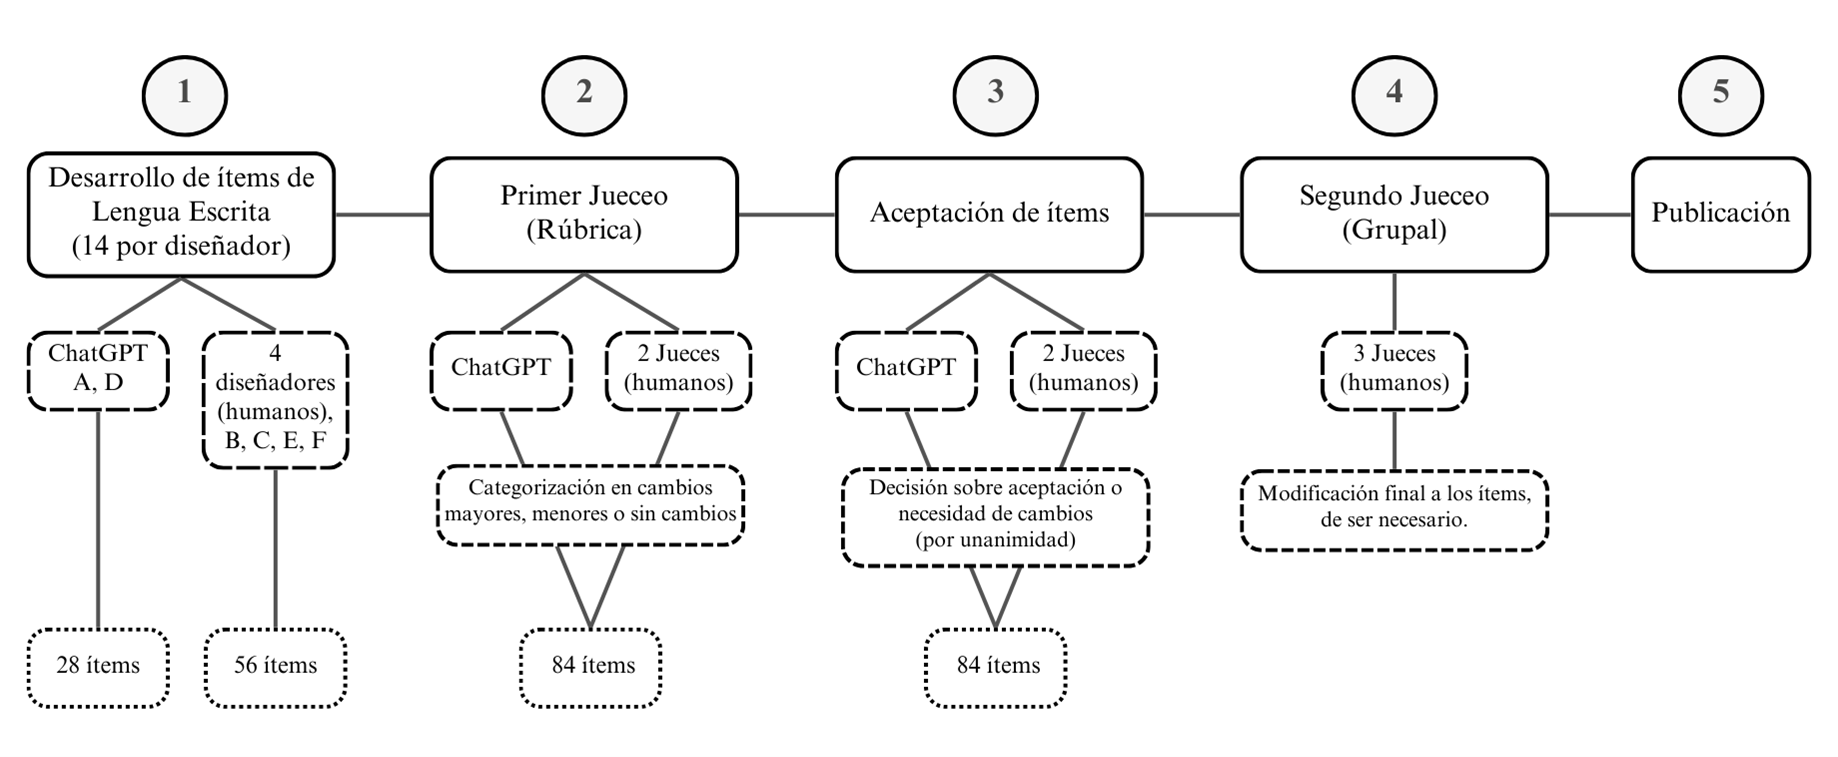
\includegraphics[width=\textwidth]{image1.png}
\caption{Proceso de evaluación y revisión de los ítems.}
\label{fig01}
\source{Elaboración propia.}
\end{minipage}
\end{figure}

Para el desarrollo de ítems se hizo uso de la IAGen ChatGPT
(\url{chat.openai.com}) en su versión de pago nombrada 4.0. Se abrieron
conversaciones por cada ítem creado, ya que todavía no estaba disponible
la posibilidad de crear un GPT con los criterios específicos para la
elaboración de ítems. En este sentido, cada ítem fue solicitado con las
características del manual de Lengua Escrita, comenzando por el uso de
la Taxonomía de \textcite{Anderson2001} para el nivel de demanda
cognitiva según la tabla de especificaciones. En cada prompt creado se
especificó:

\begin{enumerate}
	\def\labelenumi{\arabic{enumi}.}
	\item
	Identificación del contenido a evaluar
	\item
	Descripción del contenido a evaluar:
	
	\begin{enumerate}
		\def\labelenumii{\alph{enumii}.}
		\item
		Interpretación
		\item
		Ejemplos
		\item
		Delimitación del contenido
		\item
		Conocimientos y habilidades previas
		\item
		Actividades cognoscitivas
	\end{enumerate}
	\item
	Plantilla del ítem:
	
	\begin{enumerate}
		\def\labelenumii{\alph{enumii}.}
		\item
		Estructura base del ítem
		\item
		Características del texto
		\item
		Estructura y descripción de respuesta correcta y distractores.
	\end{enumerate}
	\item
	Peculiaridades de la plantilla:
	
	\begin{enumerate}
		\def\labelenumii{\alph{enumii}.}
		\item
		Base del ítem
		\item
		Vocabulario empleado
		\item
		Edición
		\item
		Peculiaridades de los distractores
	\end{enumerate}
	\item
	Bibliografía consultada y a consultar
\end{enumerate}

Por otro lado, la evaluación de los ítems fue realizada por dos jueces
humanos y por ChatGPT, siguiendo el modelo de evaluación de contenido
descrito por \textcite{Haladyna2004} y \textcite{Lynn1986}. Los jueces evaluaron cada
ítem en términos de necesidad de cambios, calidad de distractores y
aceptabilidad general del ítem. Ante esto, es importante resaltar que el
método utilizado para la evaluación de los ítems fue a doble ciego; a
ChatGPT tampoco se le indicó si quien elaboró el ítem era un ser humano
o una IAGen. Este proceso de evaluación se alinea con las
recomendaciones de \textcite{Nitko2011} sobre la importancia de una
revisión integral en la construcción de ítems de evaluación.

Los jueces evaluaron los ítems con una rúbrica (véase \Cref{tab-01}), por lo
que en esta etapa no interactuaron entre sí. Al final debían señalar si
el ítem debiese ser aceptado, aceptado con modificaciones o, bien,
podían descartarlo. Asimismo, a ChatGPT se le solicitó evaluar cada uno
de los ítems con la rúbrica disponible; es importante destacar que era
necesario tener una conversación diferente por cada ítem evaluado,
puesto que su capacidad de recordar la rúbrica era corta; es posible que
en la actualidad haya mejorado, por lo que se tiene que seguir probando
esta herramienta.



\begin{table}[!htpb]
\centering
\small
\caption{Dimensiones de la rúbrica.}
\label{tab-01}
\begin{tabular}{ll}
\toprule
Dimensiones & Elementos Clave \\
\midrule
\multirow{2}{*}{Claridad y Pertinencia del Contenido} & - Información necesaria y clara \\
    & - Tema comprensible para el público objetivo \\
\multirow{2}{*}{Neutralidad y Accesibilidad} & - Libre de sesgos\\
	& - Inclusión de imágenes/gráficas claras \\
\multirow{2}{*}{Concisión y Formato} & - Longitud adecuada del texto\\
		& - Cumplimiento de las especificaciones de formato \\
\multirow{2}{*}{Alineación Curricular} & - Congruencia con especificaciones\\
	& - Adecuación al nivel cognitivo y al público objetivo \\
\multirow{2}{*}{Claridad Disciplinar y Enfoque} & - Brevedad y claridad situacional\\
	& - Presentación directa y positiva \\
\multirow{3}{*}{Redacción y Ortografía} & - Claridad en la redacción\\
	& - Uso de vocabulario y ortografía adecuados\\
	& - Ausencia de sesgos y temas delicados \\
\multirow{3}{*}{Estructura de Respuestas} & - Uniformidad y plausibilidad de las opciones\\
	& - Ausencia de pistas indebidas\\
	& - Consistencia gramatical \\
Formato y Presentación & - Uso correcto de elementos de formato \\
\bottomrule
\end{tabular}
\source{Elaboración propia.}
\end{table}

Los resultados de las evaluaciones reflejaron una gama de decisiones,
desde la aceptación de ítems sin cambios hasta la sugerencia de
modificaciones en menor o mayor grado; o bien, el rechazo del ítem.
Estas decisiones se basaron en criterios establecidos por expertos en
evaluación educativa, como la relevancia, claridad y justicia de los
ítems \cite{Downing2003}.

Además, algunos ítems fueron seleccionados para un segundo jueceo
grupal, reflejando la metodología de revisión colaborativa sugerida por
\textcite{Stiggins2001}, lo cual permite una evaluación más profunda y detallada
en casos donde los ítems presentan desafíos particulares o requieren
ajustes más significativos. En este segundo jueceo se volvió a hacer uso
de la rúbrica, pero escuchando las observaciones de los participantes,
además se añadió a un tercer juez para tener una mejor variedad y
perspectiva sobre el jueceo.

Una vez finalizado este segundo jueceo en versión grupal, se procedió al
proceso de publicación de los ítems en su versión impresa para su
aplicación en el mes de noviembre del año 2023, como parte del proceso
de selección de ingreso a la universidad. En esta aplicación se contó
con la participación de 2,263 sustentantes, siendo 50.06~\% mujeres y
49.93~\% hombres. Los resultados de aplicación del modelo Rasch, el cual
es idóneo para medir actitudes, habilidades o personalidad
(Tristán-López, 1998), se presentan en el Anexo 1, donde todos los ítems
resultaron con índices favorables conforme a los principios de la Teoría
de Respuesta al Ítem (TRI).

Por otro lado, para el análisis del comportamiento de los jueces se
realizaron los siguientes pasos:

\begin{enumerate}[label=\Alph*)]
\item Para observar las diferencias entre el jueceo a ítems diseñados por humanos y ChatGPT
\begin{enumerate}[label=\arabic*.]
\item Preparación de datos, de forma categórica.
\item Prueba Chi-cuadrado en SPSS, siguiendo las recomendaciones de \cite{Field2013}.
\item Preparación de datos, de forma numérica para proceder a un ANOVA o
bien la prueba de Kruskal-Wallis \cite{Field2013,Howell2012}.
\item Prueba de normalidad en SPSS; el resultado fue no normal, por lo que
se procedió a la prueba de Kruskal-Wallis con las variables: Creadores
(Humano, ChatGPT), Juez A, Juez B, ChatGPT; además se aplicó la prueba
U de Mann-Whitney (Field, 2013) realizando la prueba por cada una de
las variables para revisar si había alguna variación. Todos ellos con
el \emph{software} SPSS.
\item Análisis de resultados con estadísticos básicos comparativos.
\end{enumerate}

\item Para observar la concordancia entre jueces
\begin{enumerate}[label=\arabic*.]
\item Prueba de Kappa de Cohen \cite{McHugh2012}, entre jueces: A y B, A y
ChatGPT, B y ChatGPT, a través del \emph{software} SPSS.
\item Prueba alfa de Krippendorff \cite{Hayes2007}: A, B y ChatGPT, a través del software R (Versión 2023.12.0+369), con	paquetería tidyverse e IRR.
\item Análisis de resultados con estadísticos básicos comparativos.
\end{enumerate}

\end{enumerate}
\section{Resultados}\label{sec-resultados}
\subsection{Jueceo de ítems diseñados por Humanos y ChatGPT}

Como se mencionó anteriormente, en este estudio se contemplaron dos
etapas. En este segmento se compara el resultado del jueceo según los
ítems diseñados por humanos y ChatGPT. Por un lado, se le solicitó a
ChatGPT \cite{OpenAI2023} que elaborara 24 ítems, de forma separada, pero
siguiendo los criterios marcados, y por otro, se le solicitó a cuatro
diseñadores elaborar un total de 56 ítems, 14 por cada uno de ellos. Con
el fin de evaluarlos se sometió a una revisión a doble ciego con dos
jueces humanos y un tercer juez que fue el propio ChatGPT, pero con los
parámetros de la rúbrica.

Como se describió en la metodología, se procedió a organizar la base de
datos y realizar la prueba chi-cuadrado. En la \Cref{tab-02} se pueden
observar los resultados de este primer análisis, no se observa una
diferencia significativa entre cómo evaluaron los jueces los ítems
desarrollados por humanos o por ChatGPT (Juez A, p = .758; Juez B (
.264); ChatGPT, p = 1.0). No obstante, este último, ChatGPT, muestra una
respuesta rotunda (p=1), por lo que habrá que tener cuidado sobre un
comportamiento repetitivo más que crítico.

\begin{table}[htbp]
\centering
\caption{Resultados chi-cuadrado entre ítems diseñados por humanos y
 ChatGPT según la visión de los jueces.}
\label{tab-02}
\begin{tabular}{llllp{5cm}}
\toprule
Creador & \multicolumn{1}{>{\raggedright}p{2cm}}{Chi-cuadrado de Pearson} & \multicolumn{1}{>{\raggedright}p{2cm}}{Grados de Libertad (gl)} & \multicolumn{1}{>{\raggedright}p{2cm}}{Significación Asintótica (Bilateral)} & Notas \\
\midrule
Juez\_A & 1.179 & 3 & .758 & 3 casillas (37.5~\%) tuvieron un
recuento esperado menor que 5. El recuento mínimo esperado fue .67. \\
Juez\_B & 1.247 & 1 & .264 & 2 casillas (50.0~\%) tuvieron un
recuento esperado menor que 5. El recuento mínimo esperado fue 2.33.
Solo para una tabla 2x2. \\
ChatGPT & .000 & 2 & 1.000 & 4 casillas (66.7~\%) tuvieron un
recuento esperado menor que 5. El recuento mínimo esperado fue 1.00. \\ 
\bottomrule
\end{tabular}
\source{Elaboración propia.}
\end{table}

Para complementar y teniendo los mismos resultados, se realizó la prueba
Kruskal-Wallis \cite{Field2013,Howell2012}, debido a que los resultados
de la prueba de normalidad fueron: no normal. Los resultados de la
prueba Kruskal-Wallis se observa en la \Cref{tab-03}, con los cuales se puede
confirmar que no hay diferencias significativas en las evaluaciones
(Juez\_A, Juez\_B, ChatGPT) entre los ítems creados por humanos y los
generados por ChatGPT, recordando que un valor \emph{p} menor que el
nivel de significancia elegido (0.05) indica que hay diferencias
estadísticamente significativas entre los grupos. Por ejemplo, los
resultados de Juez\_A y ChatGPT, donde los valores \emph{p} son 0.787 y
1.000 respectivamente, lo que sugiere que no hay diferencias
significativas en las evaluaciones entre los diferentes creadores de
ítems; estos resultados son similares a la realizada con chi-cuadrado
Mann Withney.

\begin{table}[htbp]
\centering
\caption{Resultados de la prueba Kruskal Wallis entre las evaluaciones de
los jueces sobre los ítems realizados entre humanos y ChatGPT.}
\label{tab-03}
\begin{tabular}{llllll}
\toprule
Variable & \multicolumn{1}{>{\raggedright}p{2cm}}{H de Kruskal-Wallis} & \multicolumn{1}{>{\raggedright}p{2cm}}{Grados de Libertad (gl)} & \multicolumn{1}{>{\raggedright}p{2cm}}{Significación Asintótica (p-valor)} & \multicolumn{1}{>{\raggedright}p{2cm}}{Prueba de la Mediana - Chi-cuadrado} & \multicolumn{1}{>{\raggedright}p{2cm}}{Prueba de la Mediana - Sig. Asintótica} \\
\midrule
Juez\_A & 0.073 & 1 & 0.787 & 0.386 & 0.534 \\
Juez\_B & 1.232 & 1 & 0.267 & 1.247 & 0.264 \\
ChatGPT & 0.000 & 1 & 1.000 & 0.000 & 1.000 \\
\bottomrule
\end{tabular}
\source{Elaboración propia.}
\end{table}

Por otro lado, se analizaron los resultados por comparación de medias,
donde se puede decir, con reservas, que los resultados del jueceo,
únicamente realizado por humanos (Juez A y B), revelan diferencias
sutiles en la aceptación de ítems entre los creados por ChatGPT y los
diseñadores humanos. En la \Cref{tab-04}, los ítems de ChatGPT mostraron una
tasa de aceptación sin cambios ligeramente superior (67.85~\%) en
comparación con los diseñadores humanos (65.17~\%). Esto sugiere que, en
términos de cumplir con los criterios establecidos inicialmente, según
los contenidos sobre Lengua Escrita, los ítems generados por ChatGPT (A
y D) se alinearon ligeramente mejor con las expectativas de los jueces.
Sin embargo, es notable que los ítems humanos (B, C, E y F) tuvieron una
tasa menor de cambios menores requeridos, pero una tasa más alta de
cambios mayores necesarios. Esto podría indicar que mientras los ítems
de ChatGPT generalmente se acercaban más a las expectativas iniciales,
los ítems humanos, cuando requerían modificaciones, necesitaban ajustes
más sustanciales.

\begin{table}[htbp]
\centering
\caption{Aceptación y comparación entre ítems realizados por humanos vs
ChatGPT (Juez A y B).}
\label{tab-04}
\begin{tabular}{lllll}
\toprule
\multicolumn{1}{>{\raggedright}p{2cm}}{Diseñadores (14 ítems por c/u)} & \multicolumn{1}{>{\raggedright}p{2cm}}{Aceptados Sin Cambios (Promedio)} & \multicolumn{1}{>{\raggedright}p{2cm}}{Aceptados Con Cambios Menores (Promedio)} & \multicolumn{1}{>{\raggedright}p{2cm}}{Aceptados Con Cambios Mayores (Promedio)} & \multicolumn{1}{>{\raggedright}p{2cm}}{Rechazados (Promedio)} \\
\midrule
%ChatGPT (A y D) & 0.6785 \textbar{} 67.8 5\% & 0.125 \textbar{} 12.5~\% & 0.1785 \textbar{} 17.85~\% & 0.0178 \textbar{} 1.7~\% \\
%Humanos (B, C, E, F) & 0.6517 \textbar{} 65.17~\% & .0625 \textbar{} 6.25~\% & .2767 \textbar{} 27.67~\% & 0.0089 \textbar{} 0.89 \% \\
ChatGPT (A y D) & 67.8 5\% & 12.5~\% & 17.85~\% & 1.7~\% \\
Humanos (B, C, E, F) & 65.17~\% & 6.25~\% & 27.67~\% & 0.89~\% \\
\bottomrule
\end{tabular}
\source{Elaboración propia.}
\end{table}

En la \Cref{tab-05}, que incluye la evaluación del Juez C (ChatGPT 4.0), se
observa un aumento en la tasa de aceptación sin cambios para ambos
grupos, siendo ligeramente más pronunciado para los ítems de ChatGPT (A
y B). Este aumento podría reflejar una alineación en la forma de evaluar
entre el ChatGPT como diseñador y como juez. Sin embargo, la tasa de
aceptación sin cambios también aumentó para los ítems humanos cuando
ChatGPT actuó como juez, lo que sugiere una evaluación consistente y
objetiva por parte de la IA. La disminución en la necesidad de cambios
menores y mayores para ambos grupos implica que el Juez C (ChatGPT) tuvo
una tendencia general a requerir menos modificaciones en los ítems.

\begin{table}[htbp]
\centering
\caption{Aceptación y comparación entre ítems realizados por humanos vs ChatGPT (Juez A, B y C).}
\label{tab-05}
\begin{tabular}{lllll}
\toprule
\multicolumn{1}{>{\raggedright}p{2cm}}{Grupo de Diseñadores} & 
\multicolumn{1}{>{\raggedright}p{2cm}}{Aceptados Sin Cambios (Promedio)} &
\multicolumn{1}{>{\raggedright}p{2cm}}{Aceptados Con Cambios Menores (Promedio)} &
\multicolumn{1}{>{\raggedright}p{2cm}}{Aceptados Con Cambios Mayores (Promedio)} &
\multicolumn{1}{>{\raggedright}p{2cm}}{Rechazados (Promedio)} \\
\midrule
%ChatGPT (A y D) & 0.7619 \textbar{} 76.19~\% & 0.0952 \textbar{} 9.52~\% & 0.1309 \textbar{} 13.9~\% & 0.0119 \textbar{} 1.19~\% \\
%Humanos (B, C, E, F) & 0.7440 \textbar{} 74.40~\% & 0.0535 \textbar{} 5.35~\% & 0.1964 \textbar{} 19.64~\% & 0.0059 \textbar{} 0.59~\% \\
ChatGPT (A y D) & 76.19~\% & 9.52~\% & 13.9~\% & 1.19~\% \\
Humanos (B, C, E, F) & 74.40~\% & 5.35~\% & 19.64~\% & 0.59~\% \\
\bottomrule
\end{tabular}
\source{Elaboración propia.}
\end{table}

No obstante, cuando se observan los resultados por diseñador, sin jueces
específicos y a partir de medias, se encuentra que no hay grandes
diferencias entre los resultados de cada uno de los diseñadores. Según
la \Cref{tab-06}, que refleja el promedio de decisiones tomadas por los tres
jueces (Juez A, Juez B y Juez C - ChatGPT 4), el 75~\% de los ítems de
todos los diseñadores fueron aceptados sin cambios, lo que indica una
alta calidad general y una alineación efectiva con los estándares de
evaluación. Este alto porcentaje de aceptación sin cambios sugiere que
la mayoría de los ítems fueron considerados adecuados y pertinentes
desde su presentación inicial. Sin embargo, hay variabilidad entre los
diseñadores, con el Diseñador B alcanzando la tasa más alta de
aceptación sin cambios (83.33~\%) y el Diseñador F la más baja (66.67
\%). Esta variación puede reflejar diferencias en los enfoques de diseño
de ítems o en la interpretación de los criterios de evaluación.

\begin{table}[!htpb]
\centering
\caption{Control de aceptación de ítems (promedio).}
\label{tab-06}
\begin{tabular}{lllll}
\toprule
\multicolumn{1}{>{\raggedright}p{2cm}}{Diseñador} & 
\multicolumn{1}{>{\raggedright}p{2cm}}{Aceptado Sin Cambios (\%)} &
\multicolumn{1}{>{\raggedright}p{2cm}}{Aceptado Con Cambios Menores (\%)} & 
\multicolumn{1}{>{\raggedright}p{2cm}}{Aceptado Con	Cambios Mayores (\%)} & 
\multicolumn{1}{>{\raggedright}p{2cm}}{Rechazado (\%)} \\
\midrule
A & 78.57~\% & 14.29~\% & 7.14~\% & 0.00~\% \\
B & 83.33~\% & 9.52~\% & 7.14~\% & 0.00~\% \\
C & 73.81~\% & 4.76~\% & 19.05~\% & 2.38~\% \\
D & 73.81~\% & 4.76~\% & 19.05~\% & 2.38~\% \\
E & 73.81~\% & 4.76~\% & 21.43~\% & 0.00~\% \\
F & 66.67~\% & 2.38~\% & 30.95~\% & 0.00~\% \\
Media & 75~\% & 6.75~\% & 17.46~\% & 0.79~\% \\
\bottomrule
\end{tabular}
\source{Elaboración propia.}
\end{table}


En cuanto a los ítems que requirieron cambios menores, la media se sitúa
en un 6.75~\%. Este porcentaje relativamente bajo indica que solo una
fracción menor de los ítems necesitaba ajustes leves para cumplir con
los criterios de evaluación. Nuevamente, existe una variación entre los
diseñadores, siendo el Diseñador B el que más a menudo requirió estos
ajustes. Los ítems que necesitaron cambios mayores presentaron una media
del 17.46~\%, lo que sugiere que, aunque en menor medida que los
aceptados sin cambios, una proporción considerable de ítems necesitó
modificaciones más sustanciales. En cuanto a la tasa de rechazo, esta
fue bastante baja, con una media del 0.79~\%, solo los Diseñadores C y D
experimentaron rechazos, aunque en una proporción mínima, lo que indica
que la gran mayoría de los ítems fueron considerados válidos y adecuados
en cierta medida.


\subsection{Consistencia y resultados entre jueces}
Sin duda, a pesar de que hubo una rúbrica como guía, como se observa en
la \Cref{tab-07}, hubo diferencias significativas entre las evaluaciones del
Juez A, B y C. El Juez A mostró un enfoque más crítico en la evaluación,
con solo un 39.29~\% de ítems aceptados sin cambios. Esta tasa más baja
sugiere un estándar riguroso o criterios más estrictos en la evaluación.
Además, un 16.67~\% de los ítems necesitó cambios menores, y una
proporción significativa, 41.67~\%, requirió cambios mayores. También se
observó un pequeño porcentaje de rechazo (2.38~\%), lo que indica que
algunos ítems no cumplían con los estándares requeridos. Por otro lado,
el Juez B adoptó un enfoque más permisivo o alineado con los diseños de
ítems, con una alta tasa de aceptación sin cambios del 92.86~\%. Esta
evaluación indulgente se refleja en la ausencia total de cambios menores
y solo un 7.14~\% de ítems que necesitaron cambios mayores. Además, no
se registraron rechazos, lo que sugiere una percepción generalmente
favorable de los ítems presentados.

\begin{table}[htbp]
\centering
\caption{Control de aceptación de ítems de los jueces.}
\label{tab-07}
\begin{tabular}{lllll}
\toprule
Juez & \multicolumn{1}{>{\raggedright}p{2cm}}{Aceptado Sin Cambios} &
\multicolumn{1}{>{\raggedright}p{2cm}}{Aceptado Con Cambios Menores} &
\multicolumn{1}{>{\raggedright}p{2cm}}{Aceptado Con Cambios Mayores} &
Rechazado \\
\midrule
Juez A & 33 \textbar{} 39.29~\% & 14 \textbar{} 16.67~\% & 35 \textbar{} 41.67~\% & 2 \textbar{} 2.38~\% \\
Juez B & 78 \textbar{} 92.86~\% & 0 & 6 \textbar{} 7.14~\% & 0 \\
\multicolumn{1}{>{\raggedright}p{2.1cm}}{Juez C (ChatGPT 4)} & 78 \textbar{} 92.86~\% & 3 \textbar{} 3.57~\% & 3 \textbar{} 3.57~\% & 0 \\
Media & 75~\% & 6.74~\% & 17.46~\% & 0.79~\% \\
\bottomrule
\end{tabular}
\source{Elaboración propia.}
\end{table}

No obstante, uno de los aspectos más relevantes fue observar la
consistencia entre los 84 ítems y los 3 jueces, el resultado fue una
concordancia baja (alfa = 0.228, véase \Cref{tab-08}), que según \textcite{Hayes2007}, el resultado varía de 0 a 1, donde valores cercanos
a 1 indican alta confiabilidad o acuerdo entre los jueces, y valores
cercanos a 0 indican lo contrario. En este sentido, como se ha analizado
anteriormente, parece existir una mayor concordancia entre el Juez B y
ChatGPT, que entre el Juez A y cualquiera de los otros dos jueces.

\begin{table}[htbp]
\centering
\caption{Resultados del alfa de Krippendorff entre los jueces.}
\label{tab-08}
\begin{tabular}{ll}
\toprule
Sujetos & 3 \\
Evaluadores & 84 \\
Alfa & 0.228 \\
\bottomrule
\end{tabular}
\source{Elaboración propia.}
\end{table}

Debido a los resultados del alfa de Krippendorf para tres jueces, se
realizó la prueba Kappa de Cohen entre los jueces A y B, y entre cada
juez y las evaluaciones de ChatGPT. Kappa de Cohen, según McHugh (2012),
es una medida de acuerdo entre dos jueces que tiene en cuenta el acuerdo
que podría ocurrir por azar. Un valor de Kappa de 1 indica un acuerdo
perfecto, mientras que un valor de 0 indica que cualquier acuerdo es
exactamente el que se esperaría por azar, y los valores negativos
indican desacuerdo. En la \Cref{tab-09} se pueden observar los resultados
entre jueces, donde:

\begin{itemize}
\item Juez A vs. Juez B: Hay un mínimo acuerdo entre estos dos jueces, que
	no es estadísticamente significativo, es decir, sus evaluaciones no
	concuerdan más allá de lo que se esperaría por azar.
\item Juez A vs. ChatGPT: Hay un mínimo, pero estadísticamente significativo
	acuerdo entre las evaluaciones del Juez A y ChatGPT. Aunque el acuerdo
	es mínimo, existe cierta concordancia más allá del azar.
\item Juez B vs. ChatGPT: Este par muestra un moderado acuerdo que es muy
	significativo estadísticamente. Indica que las evaluaciones del Juez B
	y ChatGPT concuerdan en cierta medida más allá de lo que se esperaría
	por azar. Lo que también podría significar un comportamiento
	específico a la de un humano con menos rigurosidad que, por ejemplo,
	un Juez A, más crítico.
\end{itemize}

\begin{table}[htbp]
\centering
\caption{Resultados de la prueba Kappa de Cohen entre jueces.}
\label{tab-09}
\begin{tabular}{llll}
\toprule
Comparación & Kappa & \multicolumn{1}{>{\raggedright}p{2cm}}{Significación (p-valor)} & Interpretación \\
\midrule
Juez A vs. Juez B & 0.075 & p = 0.092 & Mínimo acuerdo, no significativo \\
Juez A vs. ChatGPT & 0.089 & p = 0.017 & Mínimo acuerdo, significativo \\
Juez B vs. ChatGPT & 0.429 & p \textless{} 0.001 & Moderado acuerdo, muy significativo \\
\bottomrule
\end{tabular}
\source{Elaboración propia.}
\end{table}



\subsection{Último jueceo}
En el proceso de segundo jueceo, los resultados variaron
significativamente entre los distintos diseñadores, pero homogeneizó el
resultado final del jueceo; considerando que aquí participaron tres
jueces además del A y B y se omitió la participación de ChatGPT. En la
Tabla 6 se puede ver que para el Diseñador A, 9 de sus 14 ítems (64.29
\%) pasaron a esta etapa, con un ítem (7.14~\%) requiriendo cambios
menores y otro ítem (7.14~\%) cambios mayores, mientras que la mayoría,
7 ítems (50~\%), no necesitaron ningún cambio. De manera similar, el
Diseñador C tuvo 8 ítems (57.14~\%) en la segunda evaluación, con un
ítem (7.14~\%) necesitando tanto cambios menores como mayores, y 7 ítems
(50~\%) sin cambios. El Diseñador E también mostró un patrón parecido,
con 9 ítems (64.29~\%) en el segundo jueceo, donde 1 ítem (7.14~\%)
necesitó cambios mayores y 7 ítems (50~\%) no requirieron
modificaciones.

\begin{table}[htbp]
\centering
\caption{Resumen del control de ítems que pasaron al segundo jueceo (grupal).}
\label{tab-10}
\begin{tabular}{llllll}
\toprule
 & \multicolumn{1}{>{\raggedright}p{2cm}}{Aceptados en primer jueceo} & 
 \multicolumn{1}{>{\raggedright}p{2cm}}{Total a segundo jueceo (grupal)} &
 \multicolumn{1}{>{\raggedright}p{2cm}}{Aceptados Con Cambios Menores (Promedio)} & 
 \multicolumn{1}{>{\raggedright}p{2cm}}{Aceptados Con Cambios Mayores (Promedio)} & \multicolumn{1}{>{\raggedright}p{2cm}}{Sin cambio (Después del jueceo)} \\
\midrule
Diseñador A & 5 \textbar{} 35.71~\% & 9 \textbar{} 64.29~\% & 1	\textbar{} 7.14~\% & 1 \textbar{} 7.14~\% & 7 \textbar{} 50~\% \\
Diseñador B & 7 \textbar{} 50~\% & 7 \textbar{} 50~\% & 1 \textbar{} 7.14~\% & 0 & 7 \textbar{} 50~\% \\
Diseñador C & 6 \textbar{} 42.85~\% & 8 \textbar{} 57.14~\% & 1 \textbar{} 7.14~\% & 1 \textbar{} 7.14~\% & 7 \textbar{} 50~\% \\
Diseñador D & 4 \textbar{} 28.57~\% & 10 \textbar{} 71.43~\% & 1 \textbar{} 7.14~\% & 0 & 8 \textbar{} 57.14~\% \\
Diseñador E & 5 \textbar{} 35.71~\% & 9 \textbar{} 64.29~\% & 0 & 1 \textbar{} 7.14~\% & 7 \textbar{} 50~\% \\
Diseñador F & 3 \textbar{} 21.42~\% & 11 \textbar{} 78.57~\% & 1 \textbar{} 7.14~\% & 0 & 10 \textbar{} 71.43~\% \\
Total & 30 & 54 & 5 & 3 & 46 \\
\bottomrule
\end{tabular}
\source{Elaboración propia.}
\end{table}

Por otro lado, el Diseñador B tuvo una menor proporción de ítems que
pasaron a esta etapa, con solo 7 ítems (50~\%), y de estos, 1 ítem (7.14
\%) necesitó cambios menores y 7 ítems (50~\%) fueron aceptados sin
cambios. El Diseñador D mostró la mayor proporción de ítems en el
segundo jueceo, con 10 ítems (71.43~\%), y una alta tasa de aceptación
sin cambios, ya que 8 ítems (57.14~\%) no requirieron ajustes y solo 1
ítem (7.14~\%) necesitó cambios menores. Sobresaliendo en este proceso,
el Diseñador F presentó la mayor tasa de aceptación sin cambios, con 11
ítems (78.57~\%) pasando al segundo jueceo y 10 de ellos (71.43~\%)
aceptados tal como estaban inicialmente.

Finalmente, como se observa en la \Cref{tab-10}, la cantidad de ítems que
realmente sufrieron cambios fue un total de 8 de los 84, lo que equivale
a 9.52~\% del total. La segunda etapa de jueceo resultó muy necesaria
por la disparidad del jueceo. En este sentido, se puede concluir que el
Juez A tuvo una actitud muy crítica, lo que podría hacernos pensar en la
subjetividad del ser humano. Asimismo, en la \Cref{tab-11}, que representa el
ajuste final de los ítems después del jueceo grupal y antes de su
publicación y aplicación en un examen, se centra en los resultados
obtenidos tanto por los ítems diseñados por ChatGPT (A y D) como por los
diseñadores humanos (B, C, E, F).

\begin{table}[htbp]
\centering
\caption{Ajuste final, después de jueceo grupal, de los ítems.}
\label{tab-11}
\begin{tabular}{lllll}
\toprule
\multicolumn{1}{>{\raggedright}p{2cm}}{Grupo de Diseñadores} & 
\multicolumn{1}{>{\raggedright}p{2cm}}{Aceptados Sin Cambios (Promedio)} &
\multicolumn{1}{>{\raggedright}p{2cm}}{Aceptados Con Cambios Menores (Promedio)} &
\multicolumn{1}{>{\raggedright}p{2cm}}{Aceptados Con Cambios Mayores (Promedio)} & 
\multicolumn{1}{>{\raggedright}p{2cm}}{Rechazados (Promedio)} \\
\midrule
ChatGPT (A y D) & 85.71~\% & 7.14~\% & 3.57~\% & 3.57 \% \\
Humanos (B, C, E, F) & 89.2 8\% & 5.35~\% & 3.57~\% & 1.78 \% \\
\bottomrule
\end{tabular}
\source{Elaboración propia.}
\end{table}

Los ítems diseñados por ChatGPT mostraron una alta tasa de aceptación
sin cambios, con un 85.71~\% de los ítems considerados adecuados para su
uso sin necesidad de modificaciones adicionales. Esto indica que una
amplia mayoría de los ítems generados por ChatGPT alinearon
efectivamente con los estándares de evaluación desde su concepción
inicial. Además, un 7.14~\% de estos ítems requirieron cambios menores,
lo que sugiere que solo se necesitaron ajustes leves en una proporción
relativamente pequeña de casos. En cuanto a los cambios mayores, solo un
3.57~\% de los ítems necesitó este tipo de ajustes, y la misma
proporción (3.57~\%) fue rechazada, lo que refleja una tasa baja de
rechazo y una calidad general alta.

Por otro lado, los ítems diseñados por los diseñadores humanos
obtuvieron una tasa ligeramente superior de aceptación sin cambios,
alcanzando un 89.28~\%. Este resultado sugiere que los ítems humanos
estuvieron, en promedio, un poco más alineados con los criterios de
evaluación que los ítems de ChatGPT. Sin embargo, la diferencia no es
muy marcada, evidenciando una calidad comparable entre ambos grupos. La
tasa de ítems que requirieron cambios menores fue del 5.35~\%,
ligeramente inferior a la de ChatGPT, mientras que la proporción de
ítems que necesitaron cambios mayores fue idéntica a la de ChatGPT, 3.57
\%. La tasa de rechazo para los ítems humanos fue del 1.78~\%,
ligeramente inferior a la de ChatGPT, lo que indica un margen muy
estrecho en términos de calidad y aceptación general.

\section{Discusión}\label{sec-discusión}

Las personas entrevistadas en ambas comunas de Chile han integrado las
tecnologías digitales a sus experiencias cotidianas. Sin embargo, esas
experiencias son afectadas por las brechas digitales estructurales
existentes, lo que genera como consecuencia, limitaciones para usar
tecnologías en contextos laborales \cite[P.11]{MORALES2020}.

La tendencia a no hacer usos complejos de tecnología y concentrarse en
experiencias de entretenimiento, se conecta con investigaciones previas
respecto a los ambientes digitales como mecanismos de evasión de la
realidad y con posibles efectos negativos, que orientan hacia un uso
excesivo y unívoco de redes sociales, con posibles efectos sobre la
salud mental de los usuarios \cite{CHARITSIS2022,XU2023}. Al mismo tiempo, estas prácticas, aunque actúan como una
limitación, tienen un potencial de convertirse en herramientas para
avanzar hacia procesos de alfabetización digital más complejos, en
particular las que se vinculan con búsqueda de información o
comunicación comunitaria.

En relación con las brechas digitales y sus causas estructurales, y del
mismo modo que los trabajos previamente citados de \textcite{PETHIG2021}
o \textcite{LONGORIA2022}, puede decirse que su manifestación es
multidimensional. El contexto territorial, la desigualdad económica,
educativa y de género, entre otros factores, generan efectos
acumulativos en el mundo digital. A lo anterior se suma la propia
situación de discapacidad debido a las brechas de diseño de
dispositivos, aplicaciones y sitios web \cite{EGARD2021,KELLY2016}.

Otra cuestión preocupante es la experiencia de temor a la tecnología que
algunas entrevistadas manifestaron. A diferencia de lo señalado por
\textcite{PETHIG2021}, que asocian la tecnología a la protección frente
al miedo de exponerse a la sociedad, en las entrevistas se manifiesta un
temor a los dispositivos y a su manipulación.

En este contexto, las entrevistas en ambas comunas dan cuenta de pocas
oportunidades formales de alfabetización digital, por lo que las
experiencias de uso de tecnologías en el trabajo son limitadas,
concentrándose en aquellos que tuvieron acceso a educación
técnico-profesional. De esta forma, se manifiesta una amplia disparidad
entre las competencias laborales demandas por el mercado laboral y las
posibilidades de alfabetización disponibles en sus contextos locales. El
contexto de brechas digitales estructurales y las limitaciones de acceso
a alfabetización digital, son coincidentes con lo señalado por \textcite{QU2022}
respecto a la precarización laboral, baja calificación y remuneración.

Debido al diseño de sitios web gubernamentales que no cumplen los
criterios establecidos en las propias normativas, y de forma similar a
lo señalado por \textcite{LIN2018}, puede decirse que hay políticas de
accesibilidad, pero baja implementación. En contraste con ese déficit en
la política nacional, la accesibilidad proviene de políticas comunales
que facilitan la conectividad, y que a su vez tienen un potencial de
vinculación comunitaria, en la que las PeSD pueden acceder a internet,
espacios de encuentro comunitario y con potencial para la formación de
competencias digitales para el trabajo.

Lo anterior implica el desafío de diseñar estrategias de política para
enfrentar la inevitable penetración de las tecnologías digitales en
todos los ámbitos de la vida, y especialmente en el mundo del trabajo
\cite{PEREZROLDAN2021}.

De acuerdo con \textcite[p. 4438]{LIN2018}, la inclusión no es
exclusivamente un esfuerzo de política pública, sino más bien de
transformación de la sociedad. En ese mismo sentido apunta el trabajo de
\textcite[p. 3]{KOLOTOUCHKINA2022} que identifican cuatro
áreas para la inclusión digital: políticas de equidad digital, políticas
de estandarización, construcción de una cultura de accesibilidad
universal y compromisos sociales compartidos por el Estado, el sector
privado y la sociedad civil.

Finalmente, es importante considerar las limitaciones de la
investigación. Como se ha señalado, la investigación previa sobre PeSD y
el contexto digital laboral ha sido poco explorado, especialmente en
América latina. Es por ello que inicialmente se optó por un trabajo
descriptivo, y que requiere ser profundizado en el futuro con muestras
más amplias en otros contextos dentro del país o en América Latina y que
consideren más en detalle cuestiones como género o interculturalidad,
entre otros factores a considerar.



\printbibliography\label{sec-bib}
%conceptualization,datacuration,formalanalysis,funding,investigation,methodology,projadm,resources,software,supervision,validation,visualization,writing,review
\begin{contributors}[sec-contributors]
\authorcontribution{Karla Karina Ruiz Mendoza}[investigation,formalanalysis,writing,]
\authorcontribution{Luis Horacio Pedroza Zúñiga}[investigation,supervision,validation,review]
\authorcontribution{Alma Yadhira López García}[methodology,supervision,validation]

\end{contributors}

\appendix

\section{Anexo 1}\label{appdx1}

% Save the original values of LTleft and LTright
\newlength{\originalLTleft}
\setlength{\originalLTleft}{\LTleft}
\newlength{\originalLTright}
\setlength{\originalLTright}{\LTright}
\setlength\LTleft{-2cm}
\setlength\LTright{-2cm}
\begin{footnotesize}
\begin{longtable}{l >{\raggedright}p{2cm} *{8}{l}}
\caption{Resultados de los 28 ítems elaborados por ChatGPT 4.0}
\label{tab-12}\\
\toprule
No. & Tema & \multicolumn{1}{>{\raggedright}p{1.2cm}}{Demanda cognitiva} & \multicolumn{1}{>{\raggedright}p{1.2cm}}{Dificultad} & \multicolumn{1}{>{\raggedright}p{1.2cm}}{Infit MNSQ} & \multicolumn{1}{>{\raggedright}p{1.2cm}}{Infit ZSTD} & \multicolumn{1}{>{\raggedright}p{1.2cm}}{Outfit MNSQ} & \multicolumn{1}{>{\raggedright}p{1.2cm}}{Outfit ZSTD} & \multicolumn{1}{>{\raggedright}p{1.2cm}}{Corr. Punto-biserial} & \multicolumn{1}{>{\raggedright}p{1.2cm}}{Discriminación} \\
\midrule
	1 & Uso de palabras en oraciones & Evaluación & 0.39 & 0.93 & -0.8 & 0.85 & -1.1 & 0.35 & 1.16 \\
	2 & Uso de palabras en oraciones & Evaluación & 0.65 & 1.13 & 0.9 & 1.27
	& 1.4 & 0.01 & 0.81 \\
	3 & Uso de palabras en oraciones & Evaluación & 0.68 & 1.07 & 0.5 & 1.26
	& 1.1 & 0.04 & 0.9 \\
	4 & Uso de palabras en oraciones & Evaluación & 0.56 & 0.96 & -0.6 &
	0.96 & -0.4 & 0.32 & 1.12 \\
	5 & Economía del lenguaje & Evaluación & 0.56 & 1.05 & 0.7 & 1.07 & 0.8
	& 0.19 & 0.82 \\
	6 & Economía del lenguaje & Evaluación & 0.58 & 1.07 & 0.9 & 1.1 & 0.9 &
	0.14 & 0.79 \\
	7 & Economía del lenguaje & Evaluación & 0.55 & 1.12 & 1.8 & 1.17 & 1.9
	& 0.05 & 0.52 \\
	8 & Economía del lenguaje & Evaluación & 0.53 & 0.95 & -0.9 & 0.93 & -1
	& 0.34 & 1.23 \\
	9 & Uso efectivo de la semántica & Evaluación & 0.6 & 1.08 & 1 & 1.1 &
	0.7 & 0.13 & 0.82 \\
	10 & Uso efectivo de la semántica & Evaluación & 0.28 & 0.96 & -0.2 &
	0.82 & -0.6 & 0.25 & 1.05 \\
	11 & Uso efectivo de la semántica & Evaluación & 0.77 & 1.07 & 0.3 & 1.3
	& 0.8 & 0 & 0.93 \\
	12 & Uso efectivo de la semántica & Evaluación & 0.81 & 1.05 & 0.2 &
	1.87 & 1.6 & -0.06 & 0.92 \\
	13 & Uso efectivo de la semántica & Evaluación & 0.6 & 1 & 0 & 1.04 &
	0.3 & 0.23 & 0.98 \\
	14 & Concordancia entre sujeto y verbo & Aplicación & 0.68 & 1.05 & 0.3
	& 1.19 & 0.8 & 0.1 & 0.93 \\
	15 & Concordancia entre sujeto y verbo & Aplicación & 0.51 & 1.05 & 0.9
	& 1.06 & 0.9 & 0.18 & 0.75 \\
	16 & Concordancia entre sujeto y verbo & Aplicación & 0.51 & 0.98 & -0.4
	& 0.96 & -0.5 & 0.28 & 1.13 \\
	17 & Concordancia entre sujeto y verbo & Aplicación & 0.49 & 0.89 & -2.3
	& 0.87 & -2 & 0.42 & 1.64 \\
	18 & Concordancia entre sujeto y verbo & Aplicación & 0.48 & 0.87 & -2.4
	& 0.84 & -2.1 & 0.45 & 1.63 \\
	19 & Convenciones de puntuación: coma & Aplicación & 0.62 & 1.01 & 0.1 &
	1.1 & 0.7 & 0.2 & 0.95 \\
	20 & Convenciones de puntuación: coma & Aplicación & 0.42 & 0.94 & -0.8
	& 0.9 & -1 & 0.33 & 1.17 \\
	21 & Convenciones de puntuación: coma & Aplicación & 0.51 & 0.94 & -1.1
	& 0.93 & -1 & 0.34 & 1.31 \\
	22 & Convenciones de puntuación: coma & Aplicación & 0.57 & 1.07 & 0.9 &
	1.11 & 1 & 0.16 & 0.79 \\
	23 & Convenciones de puntuación: coma & Aplicación & 0.58 & 1.03 & 0.4 &
	1.08 & 0.7 & 0.19 & 0.88 \\
	24 & Convenciones de puntuación: interrogación & Aplicación & 0.43 &
	0.92 & -1.1 & 0.87 & -1.2 & 0.37 & 1.26 \\
	25 & Convenciones de puntuación: interrogación & Aplicación & 0.51 &
	1.01 & 0.2 & 1 & 0.1 & 0.24 & 0.96 \\
	26 & Convenciones de puntuación: interrogación & Aplicación & 0.44 &
	0.88 & -1.9 & 0.85 & -1.8 & 0.42 & 1.44 \\
	27 & Convenciones de puntuación: interrogación & Aplicación & 0.42 &
	0.88 & -1.6 & 0.84 & -1.5 & 0.42 & 1.32 \\
	28 & Convenciones de puntuación: interrogación & Aplicación & 0.63 &
	1.13 & 1.2 & 1.26 & 1.4 & 0.03 & 0.77 \\	
\multicolumn{3}{r}{Promedio general} & 0.55 & 1.00 & -0.14 & 1.06 & 0.03 & 0.22 & 1.04 \\
\bottomrule
\source{Elaboración propia.}
\end{longtable}
\end{footnotesize}
% Revert to the original values
\setlength\LTleft{\originalLTleft}
\setlength\LTright{\originalLTright}



\section{Anexo 2}
\setlength\LTleft{-0.125cm}
\setlength\LTright{-0.125cm}
\begin{footnotesize}
\begin{longtable}{llll}
\caption{Datos de las evaluaciones por creador y Juez}
\label{tab-13}
\\
\toprule
Creador & Evaluación Juez A & Evaluación Juez B & Evaluación ChatGPT \\
\midrule
	ChatGPT & 1 & 0 & 0 \\
	ChatGPT & 2 & 2 & 2 \\
	ChatGPT & 1 & 0 & 0 \\
	ChatGPT & 1 & 0 & 0 \\
	ChatGPT & 1 & 0 & 0 \\
	ChatGPT & 1 & 0 & 0 \\
	ChatGPT & 0 & 0 & 0 \\
	ChatGPT & 1 & 0 & 0 \\
	ChatGPT & 2 & 0 & 0 \\
	ChatGPT & 0 & 0 & 0 \\
	ChatGPT & 0 & 0 & 0 \\
	ChatGPT & 0 & 0 & 0 \\
	ChatGPT & 0 & 0 & 0 \\
	ChatGPT & 0 & 0 & 0 \\
	ChatGPT & 0 & 0 & 0 \\
	ChatGPT & 2 & 0 & 0 \\
	ChatGPT & 0 & 0 & 0 \\
	ChatGPT & 2 & 0 & 0 \\
	ChatGPT & 0 & 0 & 0 \\
	ChatGPT & 2 & 0 & 0 \\
	ChatGPT & 3 & 0 & 1 \\
	ChatGPT & 0 & 0 & 0 \\
	ChatGPT & 0 & 0 & 0 \\
	ChatGPT & 2 & 0 & 0 \\
	ChatGPT & 2 & 0 & 0 \\
	ChatGPT & 2 & 0 & 0 \\
	ChatGPT & 2 & 0 & 0 \\
	ChatGPT & 2 & 0 & 0 \\
	Humano & 1 & 0 & 0 \\
	Humano & 0 & 0 & 0 \\
	Humano & 1 & 0 & 0 \\
	Humano & 1 & 0 & 0 \\
	Humano & 0 & 0 & 0 \\
	Humano & 1 & 0 & 0 \\
	Humano & 0 & 0 & 0 \\
	Humano & 2 & 0 & 0 \\
	Humano & 0 & 0 & 0 \\
	Humano & 0 & 0 & 0 \\
	Humano & 0 & 0 & 0 \\
	Humano & 2 & 0 & 0 \\
	Humano & 0 & 0 & 0 \\
	Humano & 0 & 0 & 0 \\
	Humano & 1 & 2 & 2 \\
	Humano & 0 & 0 & 0 \\
	Humano & 0 & 0 & 0 \\
	Humano & 0 & 0 & 0 \\
	Humano & 0 & 0 & 0 \\
	Humano & 2 & 2 & 0 \\
	Humano & 2 & 2 & 0 \\
	Humano & 0 & 2 & 0 \\
	Humano & 0 & 0 & 0 \\
	Humano & 2 & 0 & 0 \\
	Humano & 2 & 0 & 0 \\
	Humano & 0 & 0 & 0 \\
	Humano & 3 & 0 & 0 \\
	Humano & 1 & 0 & 1 \\
	Humano & 2 & 0 & 0 \\
	Humano & 0 & 0 & 0 \\
	Humano & 0 & 0 & 0 \\
	Humano & 2 & 0 & 0 \\
	Humano & 1 & 0 & 0 \\
	Humano & 1 & 0 & 1 \\
	Humano & 0 & 0 & 0 \\
	Humano & 0 & 0 & 0 \\
	Humano & 2 & 0 & 0 \\
	Humano & 2 & 0 & 0 \\
	Humano & 2 & 0 & 0 \\
	Humano & 2 & 0 & 0 \\
	Humano & 2 & 0 & 0 \\
	Humano & 2 & 0 & 0 \\
	Humano & 2 & 0 & 0 \\
	Humano & 2 & 0 & 0 \\
	Humano & 0 & 0 & 0 \\
	Humano & 2 & 2 & 2 \\
	Humano & 2 & 2 & 0 \\
	Humano & 0 & 0 & 0 \\
	Humano & 2 & 0 & 0 \\
	Humano & 2 & 0 & 0 \\
	Humano & 2 & 0 & 0 \\
	Humano & 0 & 0 & 0 \\
	Humano & 2 & 0 & 0 \\
	Humano & 2 & 0 & 0 \\
	Humano & 2 & 0 & 0 \\
	Humano & 2 & 0 & 0 \\
\bottomrule 
\source{Elaboración propia.} \\
\addlinespace
\multicolumn{4}{l}{\footnotesize
	Sin cambio = 0; Con cambios menores = 1; Con cambios mayores = 2;
	Rechazado = 3.}\\
\end{longtable}
\end{footnotesize}


\end{document}
